\documentclass[journal,12pt,twocolumn]{IEEEtran}

\usepackage{setspace}
\usepackage{gensymb}

\singlespacing


\usepackage[cmex10]{amsmath}
\usepackage{multicol}
\usepackage{amsthm}

\usepackage{mathrsfs}
\usepackage{txfonts}
\usepackage{stfloats}
\usepackage{bm}
\usepackage{cite}
\usepackage{cases}
\usepackage{subfig}

\usepackage{longtable}
\usepackage{multirow}

\usepackage{enumitem}
\usepackage{mathtools}
\usepackage{steinmetz}
\usepackage{tikz}
\usepackage{circuitikz}
\usepackage{verbatim}
\usepackage{tfrupee}
\usepackage[breaklinks=true]{hyperref}

\usepackage{tkz-euclide}

\usetikzlibrary{calc,math}
\usepackage{listings}
    \usepackage{color}                                            %%
    \usepackage{array}                                            %%
    \usepackage{longtable}                                        %%
    \usepackage{calc}                                             %%
    \usepackage{multirow}                                         %%
    \usepackage{hhline}                                           %%
    \usepackage{ifthen}                                           %%
    \usepackage{lscape}     
\usepackage{multicol}
\usepackage{chngcntr}

\DeclareMathOperator*{\Res}{Res}

\renewcommand\thesection{\arabic{section}}
\renewcommand\thesubsection{\thesection.\arabic{subsection}}
\renewcommand\thesubsubsection{\thesubsection.\arabic{subsubsection}}

\renewcommand\thesectiondis{\arabic{section}}
\renewcommand\thesubsectiondis{\thesectiondis.\arabic{subsection}}
\renewcommand\thesubsubsectiondis{\thesubsectiondis.\arabic{subsubsection}}


\hyphenation{op-tical net-works semi-conduc-tor}
\def\inputGnumericTable{}                                 %%

\lstset{
%language=C,
frame=single, 
breaklines=true,
columns=fullflexible
}
\begin{document}


\newtheorem{theorem}{Theorem}[section]
\newtheorem{problem}{Problem}
\newtheorem{proposition}{Proposition}[section]
\newtheorem{lemma}{Lemma}[section]
\newtheorem{corollary}[theorem]{Corollary}
\newtheorem{example}{Example}[section]
\newtheorem{definition}[problem]{Definition}

\newcommand{\BEQA}{\begin{eqnarray}}
\newcommand{\EEQA}{\end{eqnarray}}
\newcommand{\define}{\stackrel{\triangle}{=}}
\bibliographystyle{IEEEtran}
\providecommand{\mbf}{\mathbf}
\providecommand{\pr}[1]{\ensuremath{\Pr\left(#1\right)}}
\providecommand{\qfunc}[1]{\ensuremath{Q\left(#1\right)}}
\providecommand{\sbrak}[1]{\ensuremath{{}\left[#1\right]}}
\providecommand{\lsbrak}[1]{\ensuremath{{}\left[#1\right.}}
\providecommand{\rsbrak}[1]{\ensuremath{{}\left.#1\right]}}
\providecommand{\brak}[1]{\ensuremath{\left(#1\right)}}
\providecommand{\lbrak}[1]{\ensuremath{\left(#1\right.}}
\providecommand{\rbrak}[1]{\ensuremath{\left.#1\right)}}
\providecommand{\cbrak}[1]{\ensuremath{\left\{#1\right\}}}
\providecommand{\lcbrak}[1]{\ensuremath{\left\{#1\right.}}
\providecommand{\rcbrak}[1]{\ensuremath{\left.#1\right\}}}
\theoremstyle{remark}
\newtheorem{rem}{Remark}
\newcommand{\sgn}{\mathop{\mathrm{sgn}}}
\providecommand{\abs}[1]{\left\vert#1\right\vert}
\providecommand{\res}[1]{\Res\displaylimits_{#1}} 
\providecommand{\norm}[1]{\left\lVert#1\right\rVert}
%\providecommand{\norm}[1]{\lVert#1\rVert}
\providecommand{\mtx}[1]{\mathbf{#1}}
\providecommand{\mean}[1]{E\left[ #1 \right]}
\providecommand{\fourier}{\overset{\mathcal{F}}{ \rightleftharpoons}}
%\providecommand{\hilbert}{\overset{\mathcal{H}}{ \rightleftharpoons}}
\providecommand{\system}{\overset{\mathcal{H}}{ \longleftrightarrow}}
	%\newcommand{\solution}[2]{\textbf{Solution:}{#1}}
\newcommand{\solution}{\noindent \textbf{Solution: }}
\newcommand{\cosec}{\,\text{cosec}\,}
\providecommand{\dec}[2]{\ensuremath{\overset{#1}{\underset{#2}{\gtrless}}}}
\newcommand{\myvec}[1]{\ensuremath{\begin{pmatrix}#1\end{pmatrix}}}
\newcommand{\mydet}[1]{\ensuremath{\begin{vmatrix}#1\end{vmatrix}}}
\numberwithin{equation}{subsection}
\makeatletter
\@addtoreset{figure}{problem}
\makeatother
\let\StandardTheFigure\thefigure
\let\vec\mathbf
\renewcommand{\thefigure}{\theproblem}
\def\putbox#1#2#3{\makebox[0in][l]{\makebox[#1][l]{}\raisebox{\baselineskip}[0in][0in]{\raisebox{#2}[0in][0in]{#3}}}}
     \def\rightbox#1{\makebox[0in][r]{#1}}
     \def\centbox#1{\makebox[0in]{#1}}
     \def\topbox#1{\raisebox{-\baselineskip}[0in][0in]{#1}}
     \def\midbox#1{\raisebox{-0.5\baselineskip}[0in][0in]{#1}}
\vspace{3cm}
\title{ Matrix Theory : Assignment 3 }
\author{Ritesh Kumar \\ Roll no. : EE20RESCH11005 }
\maketitle
\newpage
\bigskip
\renewcommand{\thefigure}{\theenumi}
\renewcommand{\thetable}{\theenumi}
\begin{abstract}
This problem is to demonstrate the way to prove the triangles are congruent and to prove a triangle as isosceles using matrix algebra.
\end{abstract}

\section{Problem}
ABC is a triangle in which altitudes BE and CF to sides AC and AB are equal. Show that 
\begin{enumerate}
	\item $\triangle$ABC $\cong$ $\triangle$ACF 
	\item AB = AC  i.e, $\triangle$ABC is an isosceles triangle.
\end{enumerate}
\section{Solution}
\subsection{part 1}
Let consider we have a triangle $\triangle$ABC. There are two altitudes BE and CF being  drawn from the vertices B and C respectively. \newline
 In $\triangle$ABE, taking inner product of sides  AE and EB we can write :
\begin{align}
\left( \vec{A-E} \right)^T \left( \vec{E - B} \right) = \norm{\vec{A - E}} \norm{\vec{ E - B}} \text{cosAEB}
\end{align}
\begin{align}
\implies \text{cosAEB} = \frac{\left( \vec{A-E} \right)^T  \left( \vec{E - B } \right)}{\norm{\vec{A - E}} \norm{\vec{E - B}}}
\end{align}
In $\triangle$ACF, taking inner product of sides AF and FC :
\begin{align}
\left( \vec{A-F} \right)^T \left( \vec{F - C} \right) = \norm{\vec{A - F}} \norm{\vec{ F - C}} \text{cosAFC}
\end{align}

\begin{align}
\implies \text{cosAFC} = \frac{\left( \vec{A-F} \right)^T  \left( \vec{F - C } \right)}{\norm{\vec{A - F}} \norm{\vec{F - C}}}
\end{align}
 In triangle $\triangle$ABC, 
 \begin{align}
 \text{cosAFC} = \text{cosAEB} \left( \text{CF} \perp \text{AB} \hspace{2pt} \& \hspace{2pt} \text{BE} \perp \text{AC}\right)    
 \end{align}
% \begin{figure}[htb!]	
% 	\centering	
% 	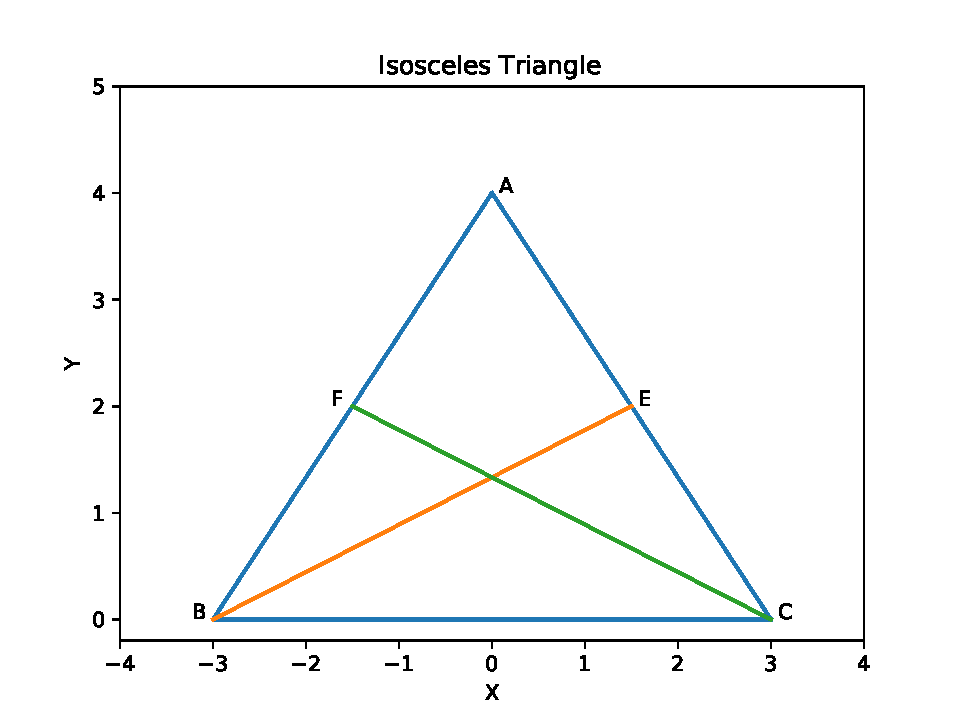
\includegraphics[width=.50\textwidth, height=.30\textheight]{Figure_1.pdf}	
% 	\caption{Isosceles triangle}
% 	\label{fig1}	
% \end{figure}
\begin{center}
\begin{tikzpicture}
\coordinate (A) at (0,6);
\coordinate (B) at (-3,0);
\coordinate (C) at (3,0);
\coordinate (E) at (1.5,3);
\coordinate (F) at (-1.5,3);
\draw (A)node[above]{$A$}--(B)node[below]{$B$}--(C)node[below]{$C$}--cycle;
\draw (B)node[below]{$B$}--(E)node[above]{$E$}--(A)node[above]{$A$}--cycle;
\draw(C)node[below]{$C$}--(F)node[above]{$F$}--(A)node[above]{$A$}--cycle;
\tkzMarkRightAngle(B,E,A)
\tkzMarkRightAngle(C,F,A)
\end{tikzpicture}
\end{center}





Given,  
\begin{align}
\norm{\vec{E - B}} = \norm{\vec{F - C}} \label{eq7}
\end{align}
\begin{align}
\angle FAC = \angle EAB \left( \text{Common angle}\right) \label{eq1.8}
\end{align}
 We know that if the two angles of triangles are equal then the third angle will also be equal.Hence,
 \begin{align}
 \angle FCA = \angle EBA  \label{eq1.9}
 \end{align}
   Hence by ASA (  Angle - Side - Angle ) We can say that , 
   \begin{align}
   \triangle \text{ABC} \cong \triangle \text{ACF}.
\end{align}
  
 
 \subsection{part 2} 
 
 we have given that ,
 \begin{align}
 	\norm{\vec{E - B}} = \norm{\vec{F - C}} \label{eq2.1}
 \end{align}
Hence we know that if the two sides of the triangle are equal then angles opposite to them are also equal. So we can have


 
Let $\textbf{m}_{AB}$ and $\textbf{m}_{CF}$ are the direction vectors of AB and CF respectively. Since AB $\perp$ CF hence,
\begin{align}
 \textbf{m}_{AB} \textbf{m}_{CF} = 0
\end{align}

\begin{align}
 \vec{\left( B - E\right)^T \left(A - C \right)} =\vec{ 0}
\end{align}
\begin{align}
\vec{\left( B -  A + A - C + C - E\right)^T \left(A - C \right)} = \vec{0}
\end{align}

  \begin{align}
 \vec{ \left( B -  A \right)^T \left(A - C \right)} + \norm{\vec {A - C}}^{2} + \vec{\left(C - F\right)^T \left(A - C \right)} = \vec{0} \label{2.5}
  \end{align}
Similarly, AC $\perp$ BE hence,  


 \begin{align}
 \textbf{m}_{AC} \textbf{m}_{BE} = 0
 \end{align}
 
 \begin{align}
 \vec{\left( C - F\right)^T \left(A - B \right)} =\vec{ 0}
 \end{align}
 \begin{align}
 \vec{\left( C -  A + A - B + B - F\right)^T \left(A - B \right)} = \vec{0}
 \end{align}
 
 \begin{align}
 \vec{ \left( C-  A \right)^T \left(A - B \right)} + \norm{\vec {A - B}}^{2} + \vec{\left(B - F\right)^T \left(A - B \right)} = \vec{0} \label{2.9}
 \end{align}
  
   In $\triangle$ABC, taking inner product of sides  AB and AC we can write :
  \begin{align}
  \left( \vec{B - A} \right)^T \left( \vec{A - C} \right) = \norm{\vec{B - A}} \norm{\vec{ A - C}} \text{cosBAC}
  \end{align}
  
 \begin{align}
\implies \text{cosBAC} = \frac{\left( \vec{ B - A} \right)^T  \left( \vec{A - C } \right)}{\norm{\vec{ B - A}} \norm{\vec{A - C}}} \label{2.11}
\end{align}  
  and,
   \begin{align}
  \left( \vec{C - A} \right)^T \left( \vec{A - B} \right) = \norm{\vec{C - A}} \norm{\vec{ A - B}} \text{cosCAB}
  \end{align}
  
 \begin{multline} 
  \implies \text{cosCAB} = \frac{\left( \vec{ C - A} \right)^T  \left( \vec{A - B } \right)}{\norm{\vec{ C - A}} \norm{\vec{A - B}}} \label{2.13}
  \end{multline} 
  
  From equation \ref{2.11}, and \ref{2.13}, we have ,
  \begin{multline} 
    \left( \vec{ B - A} \right)^T  \left( \vec{A - C } \right) =  \left( \vec{ C - A} \right)^T  \left( \vec{A - B } \right) \label{2.14}
   \end{multline} 
 using equation \ref{2.14} in \ref{2.5} and \ref{2.9} we can write,
   \begin{multline} 
   \norm{\vec{A - C}}^2 + \left ( \vec{ C - E }\right)^T \left( \vec{A - C} \right)  =  \\ \norm{\vec{A - B}}^2 + \vec{\left (  B - F\right)^{T} \left( A - B \right)}
    \end{multline} 
   
  \begin{multline} 
\norm{\vec{A - C}}^2 + \left ( \vec{ C - E }\right)^T \left( \vec{A - C} \right)  =  \\ \norm{\vec{A - B}}^2 + \vec{\left (  B - F\right)^{T} \left( A - B \right)}
 \end{multline}   
   
    \begin{multline} 
  \norm{\vec{A - C}}^2 + \left ( \vec{ C - A + A - B +B - E }\right)^T \left( \vec{A - C} \right)  =  \\ \norm{\vec{A - B}}^2 + \vec{\left (  B - A + A - C + C - F\right)^{T} \left( A - B \right)}
   \end{multline}   
  
 \begin{multline} 
\norm{\vec{A - C}}^2 +  \norm{\vec{A - C}}^2 + \left ( \vec{  A - B  }\right)^T \left( \vec{A - C} \right) + \left ( \vec{   B - E }\right)^T \\ \left( \vec{A - C} \right) =   \norm{\vec{A - B}}^2 + \norm{\vec{A - B}}^2 + \vec{\left ( A - C \right)^{T} \left( A - B \right)}  \\ +  \vec{\left (  C - F\right)^{T} \left( A - B \right)} \label{2.18}
 \end{multline}    
  
since BE $\perp$ AC and CF $\perp$ AB, hence :
\begin{align}
 \left ( \vec{   B - E }\right)^T \left( \vec{A - C} \right) = \vec{0}
 \end{align}
  and, 
  \begin{align}
   \vec{\left (  C - F\right)^{T} \left( A - B \right)} = \vec{0}
\end{align}
Now equation \ref{2.18} become :
 \begin{multline}
2\norm{\vec{A - C}}^2 + \left ( \vec{  A - B  }\right)^T \left( \vec{A - C} \right)    =  \\ 2 \norm{\vec{A - B}}^2 + \vec{\left ( A - C \right)^{T} \left( A - B \right)} \label{2.21}
 \end{multline} 

  Using equation \ref{2.14} in equation \ref{2.21},
  
  \begin{align}
  \norm{\vec{A - C} } = \norm {\vec{A - B}}
  \end{align}
  
  
  
  
  
  
\end{document}